\chapter{System Maintenance}

\section{Environment}

\subsection{Software}
\begin{itemize}
	\item Python 3
	\item IDLE
	\item PyQt 4
	\item MatPlotLib
	\item SQLite3
	\item SQLite Inspector
\end{itemize}

\subsection{Usage Explanation}
The reason I chose to use Python 3 over other languages such as C++ and Java because it is the only programming language I know in good depth, it has a syntax that is much like pseudocode, the code is much more readable than other languages such as Java, Python is widely used in professional industries and it isn't limited to a specific operating system

I chose to write my program in IDLE because it is an editor specifically designed for Python programming, it is easy to use, can be obtained easily from the official Python website, the syntax is colour coded, it makes debugging easier because errors are displayed when the program is ran and because it gets installed alongside python

The reason I chose to use PyQt 4 over other frameworks such as PySide or wxPython to make the interface is because it is the only one I know how to use, it isn't just limited to one operating system and is also relatively easy to obtain and setup. In addition to this, I used MatPlotLib within the PyQt 4 environment to make the required graphs because it integrates well with PyQt 4 and can go into it's own layout or be grouped into a layout with other widgets.

The reason I chose to use SQLite3 within Python for databasing over a flat file database or other database systems is because it is integrated well into Python by default and can be accessed just by using the line "import sqlite3" without having to install any extra modules as it is part of the standard library, it works well with Python and PyQt4 and it is widely used within professional industries.

The reason I chose to use SQLite Inspector is because it was pre-installed on the college systems so it was the easiest to access, installation at home was simple, it has a clear user interface that is easy to navigate and it allows for debugging and testing of sql statements

\subsection{Features Used}
\textbf{Python 3}
\begin{itemize}
	\item One feature from Python 3 that I used in my system was the ability to import other modules for added features and libraries on top of the basic python framework. This allowed me to use extra pieces of software alongside Python such as PyQt 4 and MatPlotLib to add the needed functionality to my system. 

	\item Another feature from Python 3 that I used was the ability to make separate classes for the different functionalities of the system and call them from other python files through the import functionality and access the methods and attributes from the parent class by instantiating it or calling it as a super class within the constructor

	\item I also used the 'pdb' module as an extra feature of Python to assist with debugging of particularly difficult problems or errors that IDLE wasn't showing logs for or where  the errors in the IDLE command line were particularly confusing.
\end{itemize}

\textbf{IDLE}
\begin{itemize}
	\item One feature of IDLE that I used was the syntax highlighting which assisted in debugging as I could tell if I had closed quotation marks properly etc.
	\item In addition to that, I also used IDLE's run functionality to test my program and debug through the ability to get errors at run time when the program crashes.
\end{itemize}

\textbf{PyQt4}
\begin{itemize}
	\item From PyQt 4 I used the QMainWindow class as a super class in my own main window to allow for easier creation of a main window interface with options such as a window title which can be changed just by calling the setWindowTitle method with the title passed in as the parameter.
	\item I also used PyQt 4's stacked layout functionality within my system to allow for multiple displays within my system without having to having to have several windows open at once and have a way to easily switch between them with buttons.
	\item A third feature from PyQt 4 that I used was it's integration with SQL through the QtSql library to allow for integration of sql into the interface. From this I was able to implement my table layout to display each database table with all the data in the table
\end{itemize}

\textbf{SQLite3}
\begin{itemize}
	\item With SQLite3 I used it's ability to save to a local database file to save the data from my system which allowed me to be able to quickly store and access any required data
	\item I also used the ability to select specific data from the database file when preparing data for my graphs so that I can have the required data displayed without having to create too many over-complicated algorithms
\end{itemize}

\textbf{SQLite Inspector}
\begin{itemize}
	\item One feature of SQLite Inspector that I used was it's ability to display data from each of my tables so that I know what's being added correctly and what is not when I'm inputting or changing data within my database
	\item Another feature I used was it's ability to run SQL statements so that I could test my sql queries before adding them to my system to make sure they worked properly
\end{itemize}

\textbf{MatPlotLib}
\begin{itemize}
	\item One specific feature of matplotlib I used was it's ability to create bar charts for displaying average data from my database
	\item Another specific feature I used was the ability to create pie charts with several tables to display the percentage consumption of the total for every consumption type in the database
\end{itemize}

\section{System Overview}

\subsection{Table Display}
The main component of the table display is a QTableView which is filled with data using a QSqlTableModel and then instantiated and added to a QStackedLayout in the main window and loaded at run time which is done with the 'show\_table' method

To switch between the database tables I implemented a QComboBox which is filled with the table names as they are pulled from the database file by calling the using an SQL query within the 'get\_tables' method and when a different table in the combo box is selected, the program identifies this change through the current index of the QComboBox changing and updates the display by calling the 'update\_table\_view' method which takes the current index of the QComboBox and then calls the 'display\_table' method which takes the table index as a parameter and sets the table of the QSqlTableModel to the given value before  selecting it's data and updating the QTableView

\subsection{Bar Chart Display}
The bar chart display is a class that is created as a child class of PyQt 4's 'QWidget' class and establishes this when defining the class and in the constructor with a function to call the constructor of the super class.

The bar chart is displayed with a Figure Canvas which is instantiated as the 'ReadingCanvas' class and added to the bar chart display as the main layout. This is then added to the main window by instantiating it and adding it to the QStackedLayout. The bar chart is displayed on the canvas by using the 'GraphController' class to get the required data through an SQL query and returning the results of the query to the bar chart class and then sending them to the 'ReadingCanvas' class as parameters of the 'show\_bar\_graph' method and using matplotlib to create the axis and draw the graph.

To switch between the different tables being displayed I used a QComboBox which the tables are added to using the 'get\_tables' method which uses an SQL query to get these tables and stores them to a list before recreating the list to have only the tables that are needed and then a for loop is used to increment through the list of tables and add them to the QComboBox in turn. The program detects when a user selects another table to be displayed from the ones listed in the QComboBox by telling when the current index of the QComboBox is changed and calling the update\_bar\_chart method which takes the selected date and table and calling the graph\_data method which gets the values from the graph controller using it's 'consumption\_averages' method with the date and table passed as parameters before sending these values to the canvas which uses the 'show\_bar\_graph' method to display the new bar graph.

\subsection{Pie Chart Display}
The pie chart display is a class which is also created as a child class of PyQt4's `QWidget' class which is called in the initialiser of the pie chart class with the line `super().\_\_init\_\_()'  The class takes the database location as a parameter when being instantiated in the main window and stores this to the variable `self.database' for easier access.

The layout for the pie chart display comprises of a QGridLayout, a QPushButton and a chart canvas inside a QVBoxLayout which is then assigned to the class which is setup as a QWidget and stored in the main window's stacked layout on instantiation.

To change the dates and/or the tables I used QComboBoxes which have the data added to them by getting the table names and dates from the database through SQL queries which are executed within the `get\_dates' and `get\_tables' methods and then added to the QComboBoxes with for loops iterating through lists. The system detects when the user changes the date or table when the index of the relevant combo box is changed and then calls the `update\_pie\_chart' method which gets the date and table combo box indexes and passes them into the `graph\_data' method which gets the totals from the `consumption\_averages' method in the `graph\_controller' class and then pases them into the `show\_pie\_chart' method in the canvas class to display the updated chart

\subsection{adding data}
The system features several windows which are all child classes of the QMainWindow class and call the super class' initialiser through the `super().\_\_init\_\_()' line in their respective initialisers. They each take the database as a parameter when instantiated in the main window class and store it to the variable `self.database'.

They each take their data using QLineEdits for text inputs, QComboBox for options where there are several set options to choose from or QCalendarWidgets for dates.

They all take their data from the input widgets and store them in local variables and then store them into the database using sql statements  which take the data as doubles or tuples depending on how much data is given or needed.

The `add\_user' class uses regular expressions for validation of the first name, last name and password and if the inputted values meet the criteria, their input boxes get a green border or if the input values are rejected the boxes get a red outline. The outlines are done by using the `setStyleSheet' method available for use with PyQt's QWidgets which take CSS strings as the parameter.

\subsection{editing data}
Editing data for each of the database tables works very similar to adding data to the tablesi in how it uses QLineEdits, QComboBoxes and QCalendarWidgets, however it also has an extra field for selecting the data to change and gets this data from the relevant table using SQL  statements which get data from the database and stores them into a list which is iterated through with a for loop and each entry added to a combobox in turn.

The validation of editing users works like adding users in how it uses regular expressions and input box highlighting.

\subsection{removing data}
Removing data works by selecting the relevant data from a QComboBox which is populated using an sql statemt to get the data from the relevant table and storing it into a list before iteratingn through it with a for loop tio add the data to the combobox

The data is removed from the database using SQL statements which take the id of the relevant data and remove the data with the matching ID.

\section{Code Structure}

\subsection{'show\_bar\_graph' method}
\begin{figure}[H]
    \pythonfile[firstline=8,lastline=26]{./maintenance/implementation/reading_canvas_class.py}
    \caption{The 'show\_bar\_graph' method} \label{python:show_bar_graph_method}
\end{figure}

This code section is part of the 'ReadingCanvas' class [See figure \ref{python:reading_canvas} on page \pageref{python:reading_canvas}]. I chose to have the 'show\_bar\_graph' method inside this class as it is what forms the bar graph canvas and therefore it makes sense to have it in the 'ReadingCanvas' class which has the base attributes which all of the graph canvases share.

The class initialiser is included in this code section because it includes the base attributes such as 'self.fig' which forms the 'page' for the graph to be drawn in and 'self.ax' which forms the graph axis that will be used by the 'show\_bar\_graph' method.

The 'data' and 'date' parameters are passed directly into the 'show\_bar\_graph' method rather than into the initialiser first because they are directly used by this method to form the graph, they aren't needed to be kept for a substantial amount of time and they can change each time the method is called.

\subsection{'GraphController' class methods}

\begin{figure}[H]
    \pythonfile[firstline=7,lastline=58]{./maintenance/implementation/graph_controller_class.py}
    \caption{The 'GraphController' class methods} \label{python:graph_controller_class_methods}
\end{figure}
These methods were put into the 'GraphController' class because they are used to get the specific data that the graphs require from the database return it. By putting them into a separate class, I can keep them all together and call them from the different classes for each of the graphs rather than put them into the different classes which eases debugging and saves me having to write the methods several times in each of the other classes.

The reason each of the methods take a date as a parameter rather than it being stored as an attribute in the initialiser is because the date provided to each of the methods can vary each time one of the methods are called so by just providing the date as a parameter rather than storing it as an attribute in the initialiser it makes it easier to allow for the date to change each time one of the methods are called.

\section{Variable Listing}
\begin{center}
	\begin{tabular}{|p{4cm}|p{4.5cm}|p{4.5cm}|}
	\hline
	\textbf{Variable name} & \textbf{Purpose} & \textbf{Location in code} \\ \hline
	path & A variable that stores the location of the database when it is taken from the QFileDialog & main\_window.py line 134 [figure \ref{python:main_window} on page \pageref{python:main_window} ]\\ \hline
	self.database\_open & A variable that stores a boolean value corresponding to whether the database is open or not &  main\_window.py line 162 [figure \ref{python:main_window} on page \pageref{python:main_window}] \\ \hline
	self.database & A variable that stores a link to the database taken from a parameter passed into the initialiser on instantiation in the main window & add\_reading\_class.py on line 10 [figure \ref{python:add_reading} on page \pageref{python:add_reading}], edit\_reading\_class.py line 9 [figure \ref{python:edit_reading} on page \pageref{python:edit_reading}] \\ \hline	
	cursor & A variable that stores a link to the database cursor & add\_reading\_class.py line 62 [figure \ref{python:add_reading} on page \pageref{python:add_reading}], edit\_reading\_class.py line 59[figure \ref{python:edit_reading} on page \pageref{python:edit_reading}] \\ \hline
	self.consumption\_types & A variable that stores a list of the consumption types that are stored in the database & add\_reading\_class.py line 64 [figure \ref{python:add_reading} on page \pageref{python:add_reading}] \\ \hline
	Type & A variable used as a counter when iterating the consumption\_types list & add\_reading\_class.py line 66,67 [figure \ref{python:add_reading} on page \pageref{python:add_reading}] \\ \hline
	Type & A variable used to store the selected consumption type before it gets added to the database & add\_reading\_class.py line 70 [figure \ref{python:add_reading} on page \pageref{python:add_reading}] \\ \hline
	Date & A variable used to store the given date before it gets added to the database & add\_reading\_class.py line 73 [figure \ref{python:add_reading} on page \pageref{python:add_reading}] \\ \hline
	sql & A variable used to store an sql query & add\_reading\_class.py line 74 [figure \ref{python:add_reading} on page \pageref{python:add_reading}] \\ \hline
	data & A variable that stores a list of data for an sql query & add\_reading\_class.py line 75 [figure \ref{python:add_reading} on page \pageref{python:add_reading}], edit\_reading\_class.py line 73 [figure \ref{python:edit_reading} on page \pageref{python:edit_reading}] \\ \hline
	readings & A variable used to store a list of the available readings in the database & edit\_reading\_class.py line 61 [figure \ref{python:edit_reading} on page \pageref{python:edit_reading}] \\ \hline
	reading & A variable used to store the selected reading & add\_reading\_class.py line 72 [figure \ref{python:add_reading} on page \pageref{python:add_reading}], edit\_reading\_class.py line 67 [figure \ref{python:edit_reading} on page \pageref{python:edit_reading}], remove\_reading\_class.py line 54 [figure \ref{python:remove_reading} on page \pageref{python:remove_reading}] \\ \hline
	\end{tabular}

	\begin{tabular}{|p{4cm}|p{4.5cm}|p{4.5cm}|}
	\hline
	new\_reading & A variable used to store the new reading that will be added to the database & edit\_reading\_class.py line 68 [figure \ref{python:edit_reading} on page \pageref{python:edit_reading} ]\\ \hline
	new\_date & A variable used to store the new date that will be added to the database & edit\_reading\_class.py line 69 [figure \ref{python:edit_reading} on page \pageref{python:edit_reading}] \\ \hline
	Cost & A variable used to store the value for the cost. & add\_cost\_class.py line 80 [figure \ref{python:add_cost} on page \pageref{python:add_cost}], edit\_cost\_class.py on line 68 [figure \ref{python:edit_cost} on page \pageref{python:edit_cost}], delete\_cost\_class.py on line 53 [figure \ref{python:delete_cost} on page \pageref{python:delete_cost}] \\ \hline
	CostID & A variable used to store the cost ID. & add\_cost\_class.py line 86 [figure \ref{python:add_cost} on page \pageref{python:add_cost}] \\ \hline
	Costs & A variable used to store a list of costs in the database & edit\_cost\_class.py line 62 [figure \ref{python:edit_cost} on page \pageref{python:edit_cost}] \\ \hline
	new\_cost & A variable used to store the new cost & edit\_cost\_class.py line 71 [figure \ref{python:edit_cost} on page \pageref{python:edit_cost}] \\ \hline
	self.name\_pattern & A variable used to store the regular expression for the name validation & add\_user\_class.py line 16 [figure \ref{python:add_user} on page \pageref{python:add_user}], edit\_user\_class.py line 17 [figure \ref{python:edit_user} on page \pageref{python:edit_user}] \\ \hline
	self.password\_pattern & A variable used to store the regular expression for the password validation & add\_user\_class.py line 17 [figure \ref{python:add_user} on page \pageref{python:add_user}], edit\_user\_class.py line 18 [figure \ref{python:edit_user} on page \pageref{python:edit_user}] \\ \hline
	password & A variable used to store the value for the password & add\_user\_class.py line 65 [figure \ref{python:add_user} on page \pageref{python:add_user}], edit\_user\_class.py line 76 [figure \ref{python:edit_user} on page \pageref{python:edit_user}] \\ \hline
	name & A variable used to store the name for validation & add\_user\_class.py line 72 [figure \ref{python:add_user} on page \pageref{python:add_user}], edit\_user\_class.py line 83 [figure \ref{python:edit_user} on page \pageref{python:edit_user}] \\ \hline
	first\_name & A variable used to store the first name & add\_user\_class.py line 86 [figure \ref{python:add_user} on page \pageref{python:add_user}] \\ \hline
	last\_name & A variable used to store the last name & add\_user\_class.py line 87 [figure \ref{python:add_user} on page \pageref{python:add_user}] \\ \hline
	User & A variable used to store the selected user & edit\_user\_class.py line 106 [figure \ref{python:edit_user} on page \pageref{python:edit_user}], remove\_user\_class.py line 53 [figure \ref{python:remove_user} on page \pageref{python:remove_user}] \\ \hline
	new\_firstname & A variable used to store the new first name & edit\_user\_class.py line 109 [figure \ref{python:edit_user} on page \pageref{python:edit_user}] \\ \hline
	new\_lastname & A variable used to store the new last name & edit\_user\_clas.py line 110 [figure \ref{python:edit_user} on page \pageref{python:edit_user}] \\ \hline
	new\_password & A variable used to store the new password & edit\_user\_class.py line 111 [figure \ref{python:edit_user} on page \pageref{python:edit_user}] \\ \hline
	users & A variable used to store a list of available users & remove\_user\_class.py line 47 [figure \ref{python:remove_user} on page \pageref{python:remove_user}] \\ \hline
	\end{tabular}
	
	\begin{tabular}{|p{4cm}|p{4.5cm}|p{4.5cm}|}
	\hline
	Type & A variable used to store the type name & add\_type\_class.py line 47 [figure \ref{python:add_type} on page \pageref{python:add_type}], edit\_type\_class.py line 69 [figure \ref{python:edit_type} on page \pageref{python:edit_type}], delete\_type\_class.py line 53 [figure \ref{python:delete_type} on page \pageref{python:delete_type}] \\ \hline
	Description & A variable used to store the type description & add\_type\_class.py line 48 [figure \ref{python:add_type} on page \pageref{python:add_type}] \\ \hline
	types & A variable used to store a list of available types & edit\_type\_class.py line 63 [figure \ref{python:edit_type} on page \pageref{python:edit_type}], delete\_type\_class.py line 47 [figure \ref{python:delete_type} on page \pageref{python:delete_type}] \\ \hline
	new\_type & A variable used to store the new type name & edit\_type\_class.py line 70 [figure \ref{python:edit_type} on page \pageref{python:edit_type}] \\ \hline
	new\_description & A variable used to store the new type description & edit\_type\_class.py line 71 [figure \ref{python:edit_type} on page \pageref{python:edit_type}] \\ \hline
	tables & A variable used to store a list of the tables & table\_layout\_class.py line 75 [figure \ref{python:table_layout} on page \pageref{python:table_layout}] \\ \hline
	table & A variable used to store the currently selected table & table\_layout\_class line 97 [figure \ref{python:table_layout} on page \pageref{python:table_layout}] \\ \hline
	totals & A variable used to store the total average consumption for the past month & bar\_widget\_class.py line 88 [figure \ref{python:bar_widget} on page \pageref{python:bar_widget}, pie\_widget\_class line [figure \ref{python:pie_widget} on page \pageref{python:pie_widget}] \\ \hline
	data\_dict & A variable to store a dictionary & reading\_canvas\_class.py line 17 [figure \ref{python:reading_canvas} on page \pageref{python:reading_canvas}] \\ \hline
	costs & A variable to store a list of costs & reading\_canvas\_class.py line 40 [figure \ref{pythin:reading_canvas} on page \pageref{python:reading_canvas}] \\ \hline
	labels & A variable to store a list of variables & reading\_canvas\_class.py line 41 [figure \ref{pythin:reading_canvas} on page \pageref{python:reading_canvas}] \\ \hline
	\end{tabular}
\end{center}

\section{System Evidence}

\subsection{User Interface}
\begin{landscape}
\begin{figure}[H]
	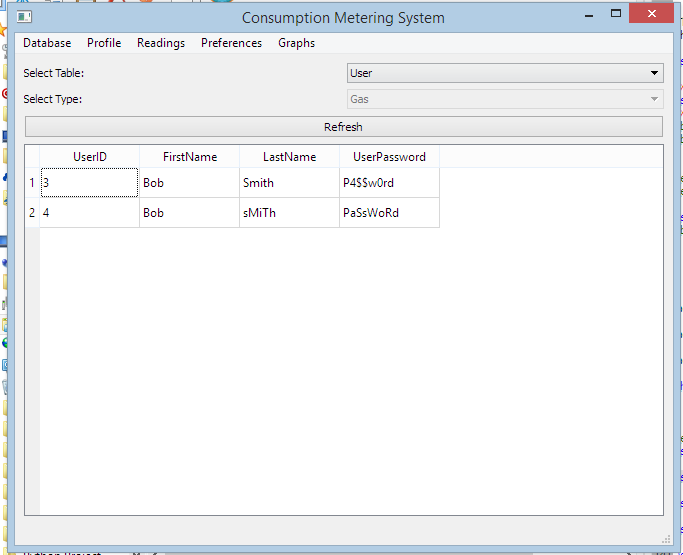
\includegraphics{./maintenance/images/UI_Table_View.png}
	\caption{Table view interface}
\end{figure}

\begin{figure}[H]
	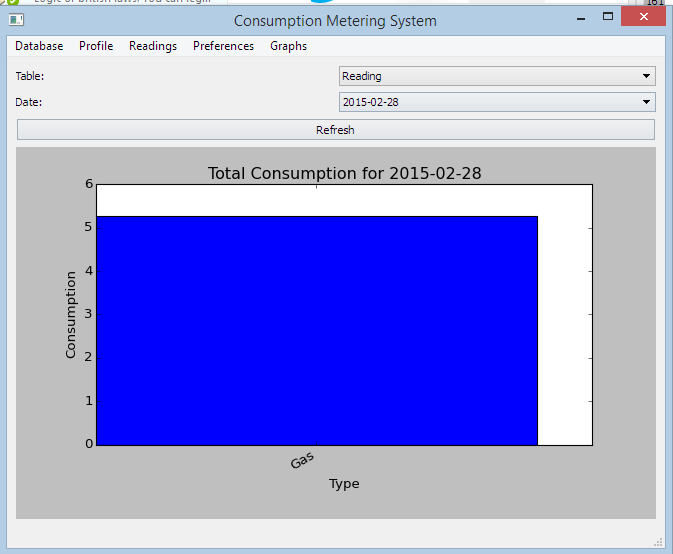
\includegraphics{./maintenance/images/UI_Bar_View.png}
	\caption{Bar chart interface}
\end{figure}

\begin{figure}[H]
	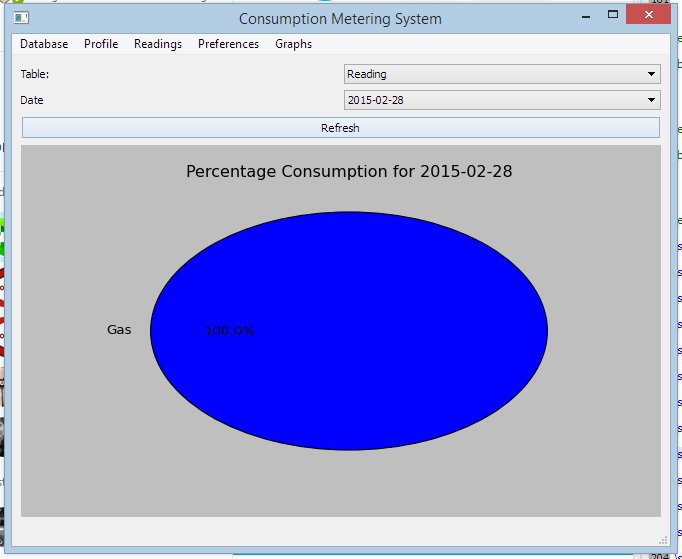
\includegraphics{./maintenance/images/UI_Pie_View.png}
	\caption{Pie chart interface}
\end{figure}
\end{landscape}

\begin{figure}[H]
	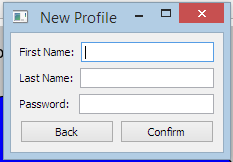
\includegraphics{./maintenance/images/UI_Add_User.png}
	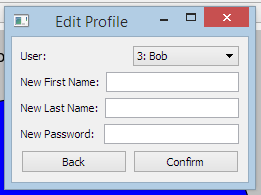
\includegraphics{./maintenance/images/UI_Edit_User.png}
	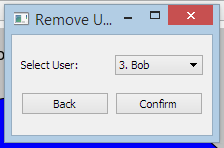
\includegraphics{./maintenance/images/UI_Remove_User.png}
	\caption{Add, edit and remove user data}
\end{figure}

\begin{figure}[H]
	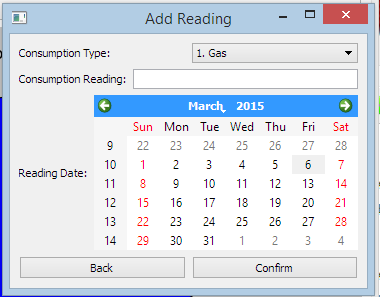
\includegraphics{./maintenance/images/UI_Add_Reading.png}
	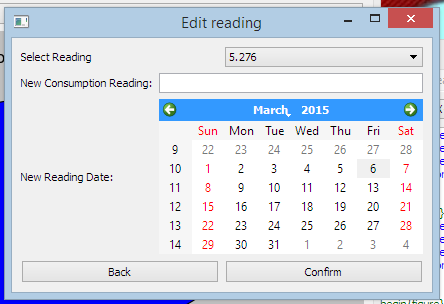
\includegraphics{./maintenance/images/UI_Edit_Reading.png}
	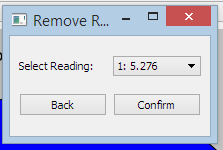
\includegraphics{./maintenance/images/UI_Remove_Reading.png}
	\caption{Add, edit and remove reading data}
\end{figure}

\begin{figure}[H]
	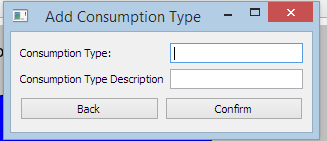
\includegraphics{./maintenance/images/UI_Add_Type.png}
	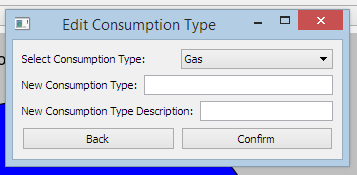
\includegraphics{./maintenance/images/UI_Edit_Type.png}
	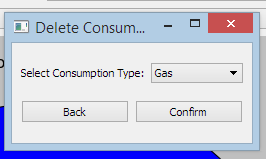
\includegraphics{./maintenance/images/UI_Remove_Type.png}
	\caption{Add, edit and remove type data}
\end{figure}

\begin{figure}[H]
	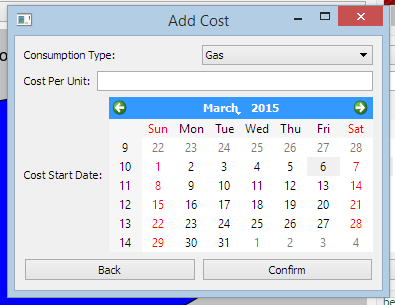
\includegraphics{./maintenance/images/UI_Add_Cost.png}
	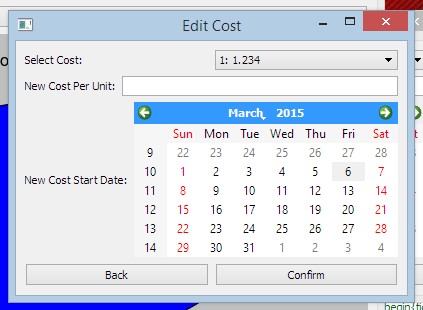
\includegraphics{./maintenance/images/UI_Edit_Cost.png}
	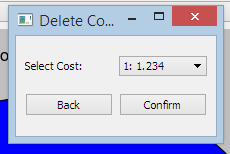
\includegraphics{./maintenance/images/UI_Remove_Cost.png}
	\caption{Add, edit and remove cost data}
\end{figure}

\subsection{ER Diagram}
\begin{figure}[H]
	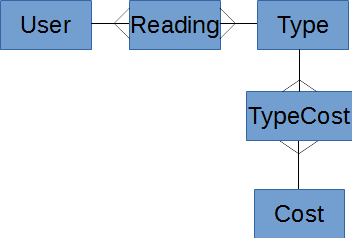
\includegraphics{./maintenance/images/ER_Diagrams.png}
	\caption{ER Diagram}
\end{figure}

\subsection{Database Table Views}
\begin{figure}[H]
	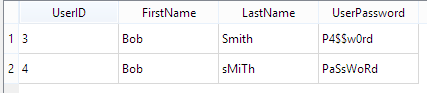
\includegraphics{./maintenance/images/User_Table_Entries.png}
	\caption{User table view}
\end{figure}

\begin{figure}[H]
	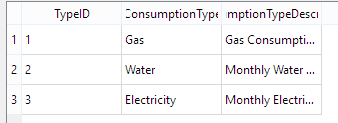
\includegraphics{./maintenance/images/Type_Table_Entries.png}
	\caption{Type table view}
\end{figure}

\begin{figure}[H]
	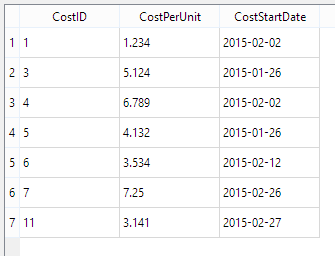
\includegraphics{./maintenance/images/Cost_Table_Entries.png}
	\caption{Cost table view}
\end{figure}

\begin{figure}[H]
	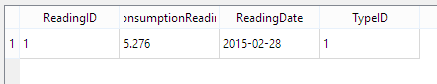
\includegraphics{./maintenance/images/Reading_Table_Entries.png}
	\caption{Reading table view}
\end{figure}

\begin{figure}[H]
	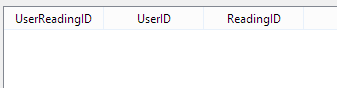
\includegraphics{./maintenance/images/UserReading_Table_Entries.png}
	\caption{UserReading table view}
\end{figure}

\begin{figure}[H]
	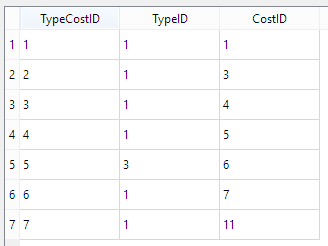
\includegraphics{./maintenance/images/TypeCost_Table_Entries.png}
	\caption{TypeCost table view}
\end{figure}

\subsection{Database SQL}
\begin{sql}
create table Type
(TypeID integer,
ConsumptionType text,
ConsumptionTypeDescription text,
primary key(TypeID))
\end{sql}

\begin{sql}
create table Reading
(ReadingID integer,
ConsumptionReading real,
ReadingDate text,
TypeID integer,
primary key(ReadingID)
foreign key(TypeID) references Type(TypeID))
\end{sql}

\begin{sql}
create table User
(UserID integer,
FirstName text,
LastName text,
UserPassword text,
primary key(UserID))
\end{sql}

\begin{sql}
create table Cost
(CostID integer,
CostPerUnit real,
CostStartDate text,
primary key(CostID)
\end{sql}

\begin{sql}
create table UserReading
(UserReadingID integer,
UserID integer,
ReadingID integer,
primary key(UserReadingID)
foreign key(UserID) references User(UserID)
foreign key(ReadingID) references Reading(ReadingID))
\end{sql}

\begin{sql}
create table TypeCost
(TypeCostID integer,
TypeID integer,
CostID integer,
primary key(TypeCostID)
foreign key(CostID) references Cost(CostID)
foreign key(TypeID) references Type(TypeID))
\end{sql}

\subsection{SQL Queries}
\begin{sql}
SELECT Type.ConsumptionType,Cost.CostPerUnit
                     FROM Type, Cost, Reading, TypeCost
                     WHERE Type.TypeID = Reading.TypeID and
                     TypeCost.CostID = Cost.CostID and
                     TypeCost.TypeID = Type.TypeID and
                     Cost.CostStartDate = Reading.ReadingDate and
                     Cost.CostStartDate = ?
                     GROUP BY Type.ConsumptionType
\end{sql}
This query gets the consumption types from the type table, the costs per unit from the cost table and compares them with data in the typecost table to make sure they correspond and then compares the date of each consumption cost per unit with a reading date to make sure they match and groups it under the consumption types before providing only data that fully corresponds with the other data that was used in comparation

\begin{sql}
SELECT avg(Reading.ConsumptionReading), Reading.ReadingDate
                     FROM Reading, Type
                     WHERE Type.TypeID = Reading.TypeID and
                     Reading.ReadingDate = ? and
                     Type.ConsumptionType = ?
                     GROUP BY Reading.ConsumptionReading
\end{sql}
This query gets an average of the consumption readings and the reading date from the reading table then compares the reading type with the provided type ID before grouping the data under the specific readings

\begin{sql}
SELECT Type.ConsumptionType,avg(Reading.ConsumptionReading) as average
                     FROM Type, Reading
                     WHERE Type.TypeID = Reading.TypeID and
                     Reading.ReadingDate = ?
                     GROUP BY Type.ConsumptionType
\end{sql}
This gets an average of the reading consumptions from the reading table and the type from the type table but only when the consumption reading's Type ID matches the Type ID and the reading's date matches the date provided when the query is executed

\section{Testing}

\subsection{Summary of Results}
From my testing I found out my system is fairly reliable and robust because most of my tests were successful and worked as expected and the program crashed very few times. [See the testing section starting on page 60]

The main weakness of my testing method was that I couldn't viably test every single possible combination for erroneous, normal and boundary data in my system as it would have taken too long and the way I tested my system made it a slow and tedious process.

The strengths of my testing method were the thorough testing of each input window to make sure it accepts data and validates data properly and the way in which I did it meant that I could easily keep track of which parts of my system I had tested, and which parts I had not tested.

\subsection{Known Issues}
Some of the known issues of my system are:
\begin{itemize}
	\item{The validation of the first name and last name - accepts special characters when it shouldn't - Possibly a problem with the regular expression}
	\item{The system doesn't reject erroneous data from the add reading window - Could be fixed by adding a regular expression for validation}
	\item{The system doesn't reject erroneous data from the add cost window - Could be fixed by adding a regular expression for validation}
	\item{The system doesn't reject erroneous data from the add type window - Could be fixed by adding a regular expression for validation}
	\item{The system doesn't edit the consumption type data properly (When just attempting to edit the consumption type name, it doesn't get changed and the consumption type description gets removed) - I am not sure how to fix this}
	\item{The system doesn't display the scatter and line graph layouts properly (graphs not generating) - I am not sure how to fix these}
	\item{The system doesn't display an option to change the table for the scatter graph - This could be fixed by adding a combobox to select the table and a method to populate this combobox and then changing the combo\_box\_layout to a QGridLayout with the select\_date\_label in position (1,1), the select\_date combo box in position (1,2) and the label and combobox for selecting the table in positions (2,1) and (2,2) respectively}
\end{itemize}

\section{Code Explanations}

\subsection{Difficult Sections}

\subsubsection{bar chart creation}
\begin{figure}[H]
	\pythonfile[firstline=15,lastline=26]{./Maintenance/Implementation/reading_canvas_class.py}
	\caption{Creation of the bar chart canvas} \label{python:bar_chart_canvas_code}
\end{figure}
The first line of this method, 'self.ax.clear()' works by clearing the axis ready to be populated with data prepared for the bar graph. Then then the data that has been passed into the method under the parameter 'data' is converted into a dictionary and stored in the variable 'data\_dict'. 

After this is done the for loop forms the bar graph with the enumerate() function taking the current value selected in the data dictionary and returns a counter value and the key corresponding to the data for each iteration of the loop. The line 'self.ax.bar(bar\_number, data\_dict[key])' constructs a single bar which is plotted onto the chart with 'bar\_number' being used as the value for the height of the bar.

'self.ax.set\_xticks(np.arange(len(data\_dict))+0.4)' sets the position of each of the 'ticks' on the x-axis to the center of their corresponding bar by adding 0.4 to their position. The value needs to be 0.4 as the default bar size is 0.8

'self.ax.set\_xticklables(list(data\_dict.keys()))' sets the labels of each 'tick' on the x-axis to the corresponding key of the data dictionary and then 'self.fig.autofmt\_xdate()' stops the labels overlapping


\subsubsection{pie chart creation}
\begin{figure}[H]
	\pythonfile[firstline=28,lastline=35]{./Maintenance/Implementation/reading_canvas_class.py}
	\caption{Creation of the pie chart canvas} \label{python:pie_chart_canvas_code}
\end{figure}
In this method, the first two lines work as they do in the 'show\_bar\_chart'. The next line, 'data = list(data\_dict.values())', works by getting the values stored in the data dictionary and stores them in a list named 'data' then the corresponding keys are stored in the 'labels' list.

Next, the line 'self.ax.pie(data,labels=labels, autopct = '%1.1f%%') creates the pie chart on the subplot  using the provided data and labels. 'autopct = '%.1.1f%%' formats the data values to 1 decimal place and then adds the percentage symbol

\subsection{Self-created Algorithms}

\section{Settings}
For this system to work the PyQt, MatPlotLib, Numpy, RE and SQLite3 modules need to be available in Python.

\section{Acknowledgements}
The regular expression used in the validation of passwords in add user [\ref{python:add_user} on page \pageref{python:add_user}] and edit user [\ref{python:edit_user} on page \pageref{python:edit_user}] came from \url{http://stackoverflow.com/questions/2990654/how-to-test-a-regex-password-in-python} in the first comment by the user 'Amber'

\section{Code Listing}
\begin{landscape}
\subsection{Main Window}
\pythonfile{./Maintenance/Implementation/new_main_window.py} \label{python:main_window}

\subsection{Add Reading Class}
\pythonfile{./Maintenance/Implementation/add_reading_class.py} \label{python:add_reading}

\subsection{Edit Reading Class}
\pythonfile{./Maintenance/Implementation/edit_reading_class.py} \label{python:edit_reading}

\subsection{Remove Reading Class}
\pythonfile{./Maintenance/Implementation/remove_reading_class.py} \label{python:remove_reading}

\subsection{Add Cost Class}
\pythonfile{./Maintenance/Implementation/add_cost_class.py} \label{python:add_cost}

\subsection{Edit Cost Class}
\pythonfile{./Maintenance/Implementation/edit_cost_class.py} \label{python:edit_cost}

\subsection{Delete Cost Class}
\pythonfile{./Maintenance/Implementation/delete_cost_class.py} \label{python:delete_cost}

\subsection{Add User Class}
\pythonfile{./Maintenance/Implementation/add_user_class.py} \label{python:add_user}

\subsection{Edit User Class}
\pythonfile{./Maintenance/Implementation/edit_user_class.py} \label{python:edit_user}

\subsection{Remove User Class}
\pythonfile{./Maintenance/Implementation/remove_user_class.py} \label{python:remove_user}

\subsection{Add Type Class}
\pythonfile{./Maintenance/Implementation/add_type_class.py} \label{python:add_type}

\subsection{Edit Type Class}
\pythonfile{./Maintenance/Implementation/edit_type_class.py} \label{python:edit_type}

\subsection{Delete Type Class}
\pythonfile{./Maintenance/Implementation/delete_type_class.py} \label{python:remove_type}

\subsection{Table Layout Class}
\pythonfile{./Maintenance/Implementation/table_layout_class_new.py} \label{python:table_layout}

\subsection{Bar Widget Class}
\pythonfile{./Maintenance/Implementation/bar_widget_class.py} \label{python:bar_widget}

\subsection{Pie Widget Class}
\pythonfile{./Maintenance/Implementation/pie_widget_class.py} \label{python:pie_widget}

\subsection{Scatter Widget Class}
\pythonfile{./Maintenance/Implementation/scatter_widget_class.py} \label{python:scatter_widget}

\subsection{Line Widget Class}
\pythonfile{./Maintenance/Implementation/line_widget_class.py} \label{python:line_widget}

\subsection{Reading Canvas Class}
\pythonfile{./Maintenance/Implementation/reading_canvas_class.py} \label{python:reading_canvas}

\subsection{Graph Controller Class}
\pythonfile{./Maintenance/Implementation/graph_controller_class.py} \label{python:graph_controller}
\end{landscape}